\documentclass[a4paper,12pt]{article}
\usepackage[margin=0.5in]{geometry} % Reduced margins
\usepackage{dmasproject}
% if you need additional LaTeX packages, add them here
\usepackage{pythonhighlight}
\usepackage[utf8]{inputenc}
\usepackage[english]{babel}
\usepackage{csquotes}
\usepackage{listings}
\usepackage{color}  % Optional for custom colors
\usepackage{caption}
\usepackage{graphicx}
\usepackage{booktabs} % For formal tables
\usepackage{wrapfig}
\usepackage{placeins}
\usepackage{pdflscape}
\usepackage{amsmath}
\usepackage[
backend=biber,
]{biblatex}

\usepackage{listings}
\usepackage{algorithmic}
\usepackage{subfig}
\usepackage{color} %red, green, blue, yellow, cyan, magenta, black, white
\usepackage{fancyvrb}
% \addbibresource{sources.bib}
\title{STAT 3400 Project Paper 2 - US Census 1840}
\author{Rudi Herrig \and Jordan Kim}
\date{May 1, 2024}

\begin{document}

\pagenumbering{arabic}

\newgeometry{left=1in,right=1in,top=1in,bottom=1in}

\definecolor{mygreen}{RGB}{28,172,0} % color values Red, Green, Blue
\definecolor{mylilas}{RGB}{170,55,241} 





\lstset{
  language=R,
  basicstyle=\ttfamily\small,
  commentstyle=\color{green},
  keywordstyle=\color{blue},
  numbers=left,
  numberstyle=\tiny\color{gray},
  stepnumber=1,
  numbersep=5pt,
  backgroundcolor=\color{white},
  frame=single,
  captionpos=b,
  breaklines=true,
  breakatwhitespace=false,
  showspaces=false,
  showstringspaces=false,
  showtabs=false,
  tabsize=2
} 




\begin{titlepage}
    \begin{center}
        \vspace*{2in}
            \huge
            \textbf{Project Paper 2}\\
             Based on 1840 data collected by the U.S. Census\\
        
        \vspace*{2 in}
        
            \normalsize
                \textbf{Rudi Herrig} \\
                \textbf{Jordan Kim} \\
                
                
        \vspace*{0.5in}
        
            STAT 3400\\
            University of Colorado Boulder\\
            Spring 2024
        
    \end{center}
\end{titlepage}



\section{New Response Variable: ACKY=ACK001/ACY\footnote{ACY is the Total White Population. \lstinline{ACKY=ACK001/ACY, \# ACKY is the Percentage of White Illiteracy}}}
\newline
Previously in our project, we used the response variable ACX001, which measures whether a county borders on a navigable waterway. Upon reflection (both ours and Dr. Pruitt's), we discovered that this variable is not random, as it measures a set-in-stone geographic fact. As such, we have pivoted to a new response variable, ACKY, which measures the illiteracy rate of white persons in the county. This variable ranges from 0 (full literacy) to 1 (full illiteracy). Unlike our previously chosen ACX001, which was a binary response variable for logistic regression using classification, our new response variable is a continuous numerical variable (percentage), so we use regression modeling in our endeavor.


\section{Cross-Validation Methodology}
In our selection processes for the lasso and ridge regression, we used a 5-fold cross-validation to test the models and find the best lambda value for the lasso and ridge regression. We then measured the accuracy of the resulting lasso model with the fixed lambda we produced using a simple validation set approach, training the model on 75 percent of the data and testing it on 35\%.

\section{Model Selection Methodologies: Lasso, Ridge, OLS, and Forward Step-Wise (AIC)}
We attempted the model selection methodologies we learned this semester, but only ended up with lasso and ridge regression as being practically useful (degree of RMSE reduction to justify). Best subset selection took over 12 hours of running before it was terminated with no output result, as our dataset includes 460 predictor variables.\footnote{Running \lstinline{best_subset <- regsubsets(ACKY~.-STATE,data=train,method="exhaustive", nvmax=200, really.big=TRUE)} repeatedly re-attempted the process with message "Reordering variables and trying again:"}
Our dataset exposes the real-world limits of best-subset selection, as it had to compare over $2^{460}$, or roughly $2.97 * 10^{138}$ different models. In order to attempt best subset selection, we would need to hand-prune our dataset to include only the predictors we think would be most significant.\footnote{Jordan wanted to try, but didn't finish through: \lstinline{train_bestsubset <- train \%\>\%
  dplyr::select(ACKY, ACD001, ACN001, ACY, ACZYZ, ACH, ACI, ACL, ACM, AC1001, AC1002, AC1, ACE, AC3, AC9M, AC9C, AC9MF, ACS, ADAF, ADAMF, ADAM, ADCM, ADCC, ADCMFF, ADCMFT, ADCMFTH, ADCMFL, ADCMFSCL, ADCMFC, ADCMFGE, ADCMFFP, ADCMFPP, ADCMFO, ADEM, ADEC, ADEMF, AC5, AB2, AB5, AB8, ACSW, ACSNW, ACSP, ACSWP, Confederate)}}    
  We also attempted forward step-wise selection, but were unable to apply it to a glm model. We tried to get around the limitations of the `olsrr` package by using step\_AIC() from the MASS package, which uses AIC instead of adjusted R2 values, and it gave us a model with only two predictor variables, Total Number of Livestock: Cattle and Total Amount of Farm Products Produced: Cotton, silk, sugar, etc.: Cotton (pounds). As seen below, neither of these variables are present in the final lasso regression model, revealing that the variables with the strongest individual connections to a predictor variable can lose their significance in larger models that also attempt to reduce variance.

We compared the lasso and ridge regression models, as well as the linear regression model with all the variables included as predictor variables. This ordinary least-squares model functioned as a good benchmark to test our shrinkage regression models against. We also use the null model as a benchmark. Our null model was the mean white illiteracy rate of all the counties in the training set, which was approximately 0.14. This null model gave us a testing RMSE of 0.138. 

\subsection{Shrinkage Methods: Lasso and Ridge Regression}
We landed on using lasso and ridge regression. The lasso regression selection methodology is particularly well-suited to our dataset, as it can cut predictor variables from the full model. Considering our 400+ potential predictor variables, lasso model is tremendously helpful with its variable selection property.
In order to find our lasso model, we conducted a 5-fold cross-validated best-lambda method.
\subsubsection{CV-Lambda Plot}
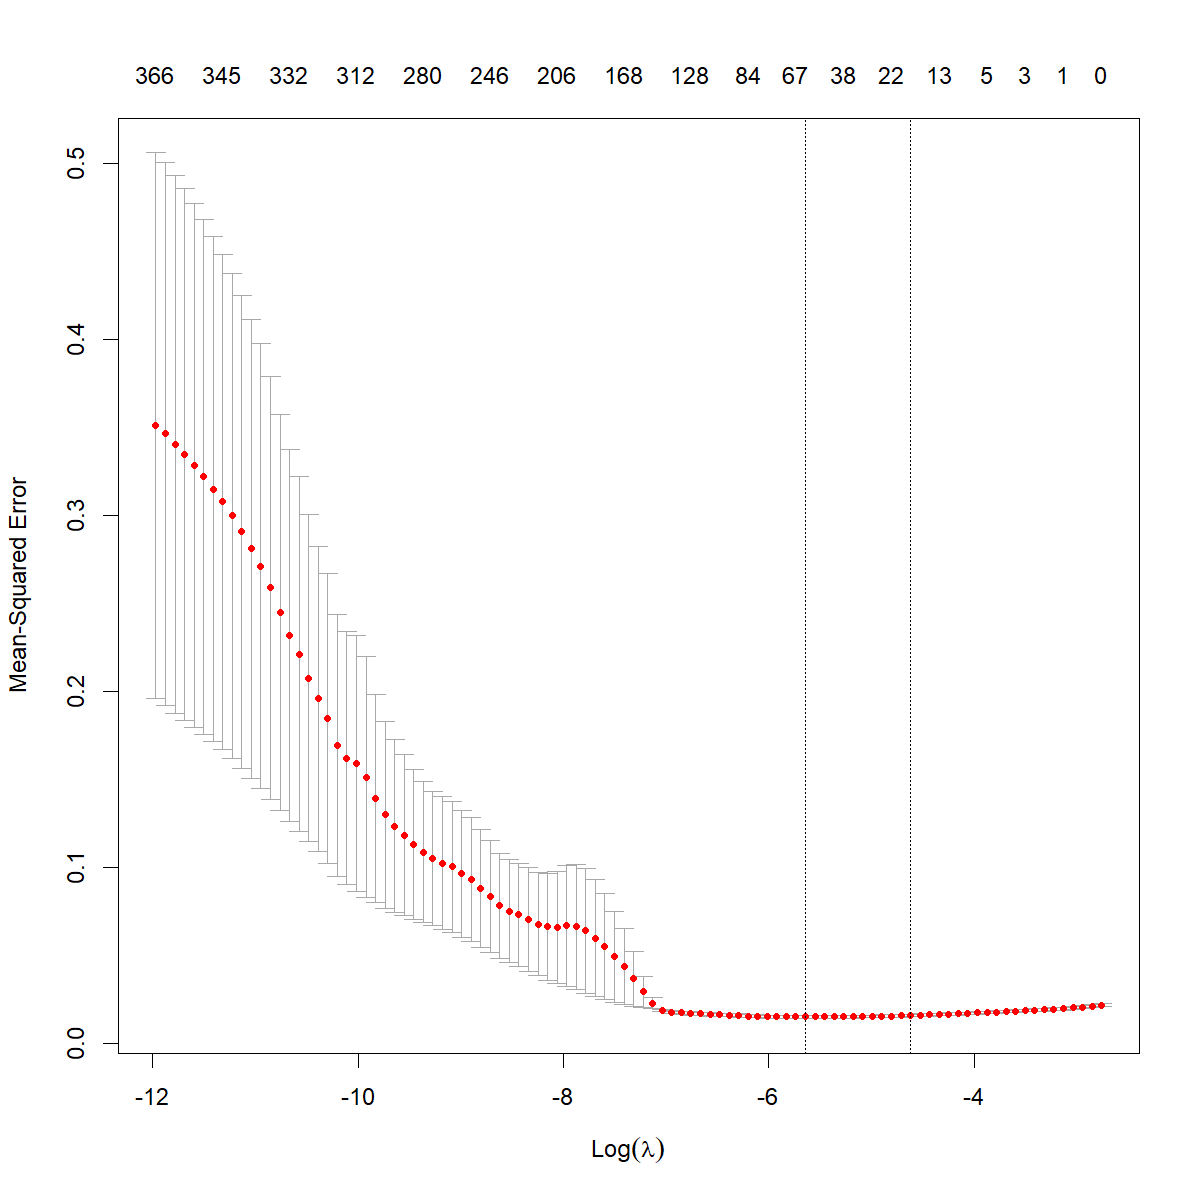
\includegraphics[scale=0.6]{cvplot.png}

As seen in the CV-Lambda plot, the RMSE values are the lowest for lasso models in the 10 to 35 predictor variables range. And our best lambda was $0.006191386$.
Using this lambda value, we calculated the testing RMSE of our lasso model, and our ridge model.

\section{Predictor Variables}
The final model created from using the lasso modeling left us these predictor variables:

\begin{itemize}
    \item - ACZ015 - Slave >> Male >> 24 to 35 years of age
    \item - ACM002 - Weekly newspapers
    \item - ACX001 - 0=NO 1=YES (Navigable Waterway)
    \item - AC9022 - Total Number of Establishments: Manufacturing: Mills: Flouring mills
    \item - AC9023 - Total Number of Establishments: Manufacturing: Mills: Grist mills
    \item - AC9027 - Total Number of Establishments: Manufacturing: Distilled and Fermented Liquors: Distilleries
    \item - ADA015 - Total Value of Production of Establishments: Manufacturing Products: Earthenware manufactured articles
    \item - ADB028 - Total Produced Number of Printing and Binding: Weekly newspapers
    \item - ADC037 - Capital Invested in Manufacturing Establishments: Mills
    \item - AB4009 - Various crops: Beeswax (pounds)
    \item - AB7008 - Various crops: Hops (pounds)
    \item - AB7013 - Various crops: Hemp (tons)
    \item - AB7020 - Cotton, silk, sugar, etc.: Cane sugar (pounds)
    \item - AB9001 - Estimated total crop output value

\end{itemize}


This model uses only 14 predictor variables, a significant reduction from the 460 of the full model. 



\section{Model Performance}
Not surprisingly, the lasso model had the best test RMSE, with an accuracy of  0.1248. Ridge Regression the next best, with an testing accuracy of 0.152. The full ordinary least-squares model had a testing RMSE of 0.75, substantially worse than all of the other models. Our lasso model performed slightly better than the null model, which indicates that our model gets roughly 1 percent closer to the actual illiteracy rate than our null model. One significant observation to note is that the the ridge regression model was significantly better than the least squares model, even though they both included all the predictors. This suggests that the lowered variance in the ridge regression significantly outweighed the increase in bias. 
When we finally used our lasso model to assess the accuracy using all of the data, the RMSE was $0.1184195$.


The forward-stepwise selection model with only two predictor variables performed surprisingly well, with an RMSE of $0.1361$.



\section{Most Valuable Predictor}
Our most valuable predictor variable seemed to be ACZ015, which measures the county's total population of male slaves aged 24 - 35. This variable has a strong positive coefficient, indicating that the population of slaves had a positive correlation with the white illiteracy rate. This variable being the predictor variable with the largest absolute value coefficient reveals the bundle of economic, cultural, and educational differences between the free and slave states of the United States in the decades leading up to the Civil War, foreshadowing their eventual split.


\section{Real-World Applications and Benefits}
Our model offers real-world applications, though its effectiveness may seem counterintuitive at first. The minimal improvement over the null model highlights the significant variability among individual counties and the modest impact of economic and industrial factors on 1840s illiteracy rates. Despite these limitations, the predictive regression model can still provide insights into the relationships between illiteracy rates and other factors during that period, which could prove valuable for economic historians in their research.
\subsection{Visualization has Benefits}
To demonstrate how our model could aid economic historian's research, I've created the image below.
\begin{figure}[ht]
\centering
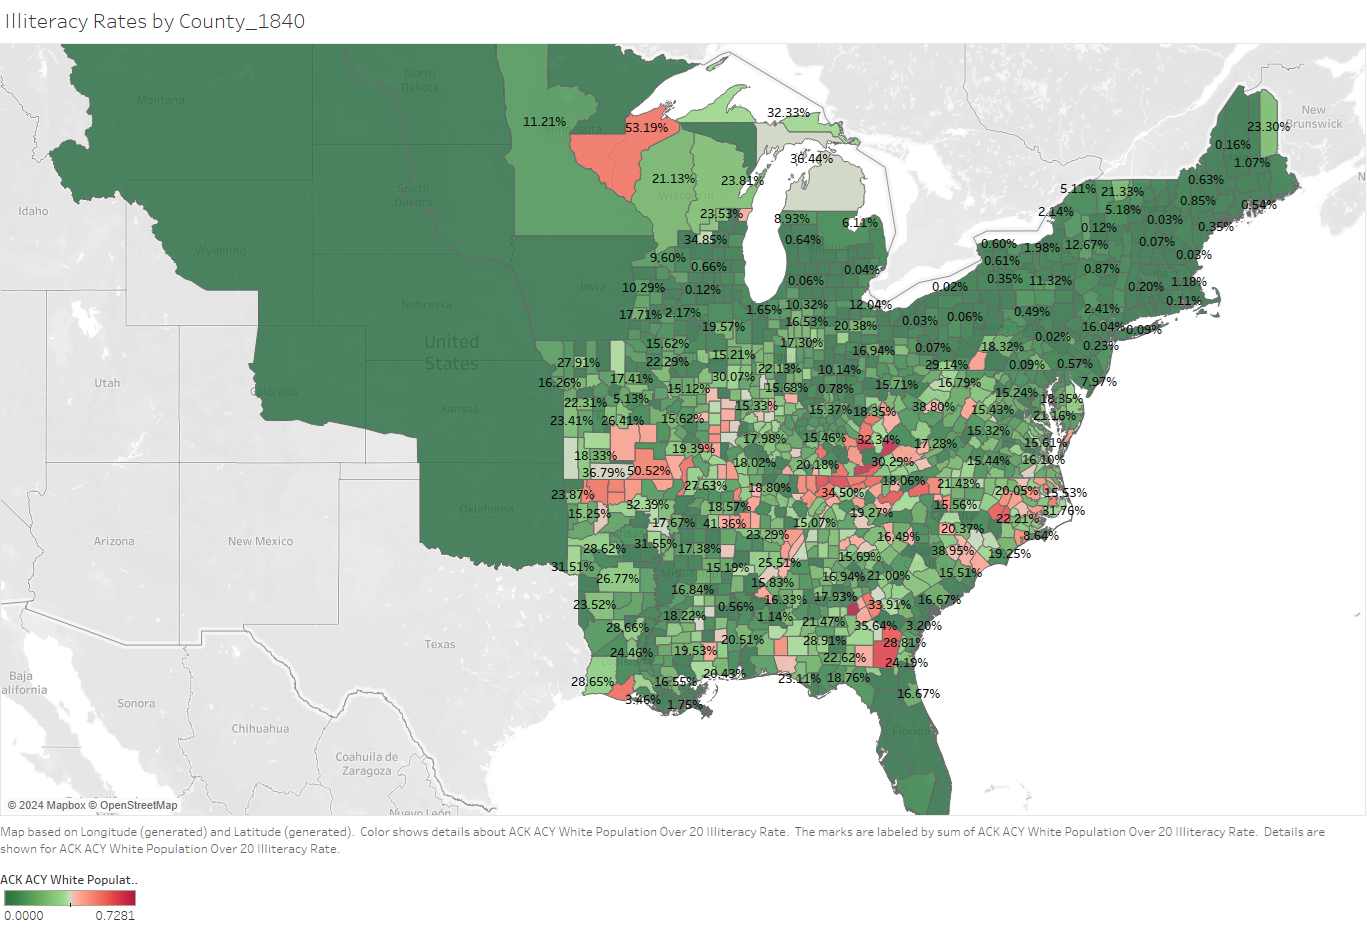
\includegraphics[scale=0.35]{IlliteracyRatesByCounty_1840.png}
\caption{I created a tableau map of our dataset with County borders drawn and color-gradient-coded into Union counties and Confederate counties and labeled with Illiteracy Rates as percentages (\%).}
\label{fig:IlliteracyRatesByCounty_1840}
\end{figure}
\newline
As seen in the map, the majority of counties in the North had low illiteracy rates among Whites.\footnote{See Appendix for larger image.}
We also include plots of other economic variables that implies and would indicate an underlying relationship with what our Response Variable measures, the ability to read and write. Such economic variables, which were to be useed in our best subset selection model, include ACH, ACI, ACM.\footnote{Please see Appendix for these plots.}
ACI is the Total Learning Institutions in the county, ACI measured Total Number of Students, and ACM was an aggregated sum of "Number of Newspapers and Periodicals" that were in circulation in the county,
\FloatBarrier % Ensure that all figures are placed before this point
\subsection{Concluding Remarks}
Our model did uncover a significant connection between a county's slave population ratio and white illiteracy rate. One could argue that this illustrates how negative effects of the slave-based economy and plantation system spread far beyond just the people it most oppressed, the slaves, but also enslaves the masters themselves into higher illiteracy which is culturally destructive. The plots in the Appendix, which show the contrast between southern and northern states and the connection between white illiteracy rates and various predictor variables, are good examples of how our data analysis could be utilized to paint the historical economic scenes in counties across the nation in a historian's research into economic factors.\footnote{\*If we may pose some philosophical questions, is a county's illiteracy rate dependent on the population's racial makeup? Or is a county's illiteracy rate being associated with the racial and free-slavery compositions of its population an observable consequence of the economic activities taking place in the county and whether the primary occupations in any given county require literacy? Could it be like asking if the chicken or the egg came first? \#FoodForThought}

If we could use time series data, it would unlock a whole new world into another dimension, offering potential pathways to a plethora of research ideas, applications, and insights. Time series analysis could allow us to track changes over time, identify trends, and build forecasting models (for other civilizations from history, illiteracy is no longer as prevalent and isn't a serious issue for most of the world.) based on historical patterns. This capability would be particularly valuable for examining how variables such as literacy rates, employment statistics, or economic factors evolve, enabling us to make more dynamic and predictive assessments. Moreover, time series data could facilitate a deeper understanding and enable theorizing upon the cause-and-effect relationships among various socioeconomic indicators. Ultimately, incorporating time series analysis could transform static snapshots of data into vibrant, evolving narratives that better reflect the complexities of societal progress and challenges. But we accept this trade-off in project complexity and scope for simplicity, interpretability, and clarity in our current analysis.


%\normalsize
\newpage
\appendix

\section{Code}
\subsection{CV-best-lambda and Lasso Model}
\begin{lstlisting}
#load glmnet library
library(glmnet)
set.seed(303)
lambda_cv <- cv.glmnet(x=x_train,y=y_train,family="gaussian",alpha=1,nfolds=5)
plot(lambda_cv)
lambda_best <- lambda_cv$lambda.min
lambda_best
model_lasso <- glmnet(x=x_train,y=y_train,family="gaussian",standardize=TRUE,alpha=1)
set.seed(303)
# testing lasso rmse
test_pred_lasso <- predict(model_lasso,newx=x_test,s=lambda_best,type="response")

RMSE_lasso=sqrt(mean((test$ACKY-test_pred_lasso)^2))
RMSE_lasso

# building full lasso model using all data
set.seed(303)
#convert all sample data to matrix form
x_all <- model.matrix(ACKY~.,data=alldata)[,-1]
y_all <- alldata$ACKY

#fit lasso model using all sample data
model_best <- glmnet(x=x_all,y=y_all,family="gaussian",standardize=TRUE,alpha=1)

#view coefficients for best model
lasso_coefficients <- predict(model_lasso,type="coefficients",s=lambda_best)
lasso_coefficients
\end{lstlisting}

\subsection{Ridge and OLS}
\begin{lstlisting}
set.seed(303)

model_ridge <- glmnet(x=x_train,y=y_train,family="gaussian", standardize=TRUE, alpha=0)
model_ols <- glm(ACKY~.,data=traindata,family="gaussian")
# testing ordinary least squares and ridge regression model RMSE
test_pred_ols=predict(model_ols,newdata=test,type="response")
test_pred_ridge=predict(model_ridge,newx=x_test,s=lambda_best,type="response")

RMSE_ols=sqrt(mean((test$ACKY-test_pred_ols)^2))
RMSE_ols
RMSE_ridge=sqrt(mean((test$ACKY-test_pred_ridge)^2))
RMSE_ridge
\end{lstlisting}
\subsection{Forward Stepwise using AIC}
\begin{lstlisting}
# Load the MASS package
library(MASS)
set.seed(303)
#define the ols model
model <- glm(ACKY~.-STATE-STATEICP-COUNTY,data=train, family = "gaussian")

# Perform forward stepwise model selection using stepAIC
stepwise_model <- stepAIC(model, direction = "forward", trace = 1)

# Review the selected model
model_summary <- summary(stepwise_model)

# Extract the coefficients table from the summary
coefficients_table <- model_summary$coefficients

# Filter for significant coefficients at the 99% confidence level
significant_coefficients <- coefficients_table[coefficients_table[, "Pr(>|t|)"] < 0.01, ]

# Print significant coefficients
print(significant_coefficients)
\end{lstlisting}

\section{Code Output}
\subsection{Forward Stepwise Model Coefficients}
\begin{lstlisting}
            Estimate   Std. Error   t value     Pr(>|t|)
AB2002  4.245243e-06 1.315045e-06  3.228211 1.312053e-03
AB4017 -5.002397e-05 9.664333e-06 -5.176143 3.073287e-07
\end{lstlisting}

\subsection{Lasso Model Predictor Variables and Coefficients}
Coefficient names and values in our final model, we omit the variables whose coefficients are reduced to 0 using the lasso method.       
\begin{table}[h]
\centering
\begin{tabular}{lr} % Aligns the first column to the left and the second to the right
\toprule
Coefficient Name & Value \\
\midrule
ACZ015 & 0.291287386134442 \\
AC3001 & -3.44181433450266e-05 \\
ACF003 & 0.000866090191803322 \\
ACH001 & 0.000682547264910997 \\
ACH003 & -0.00149940331402961 \\
ACM002 & -1.74713774127698e-05 \\
ACX001 & -0.00302409705788793 \\
AC9021 & -0.0129767702188326 \\
AC9022 & -0.000920711789329719 \\
AC9023 & -0.00067777561761586 \\
AC9027 & 0.0003727920827949 \\
ADA015 & 0.000309713100456261 \\
ADB003 & -4.57146756471891e-08 \\
ADB004 & 2.88048404034715e-09 \\
ADB028 & 3.89378808602684e-07 \\
ADE007 & -1.40516214926516e-06 \\
AB2004 & 5.39073560065452e-05 \\
AB4001 & 9.57964156974407e-08 \\
AB4009 & -9.90148903567185e-09 \\
AB7005 & 2.04416395241444e-05 \\
AB7008 & -0.000101393216259018 \\
AB7011 & -0.092503698230702 \\
AB7013 & -0.0184123409790051 \\
AB7020 & -0.00142841365128083 \\
AB8005 & 0.000176851941959287 \\
AB8010 & -1.92870365287544e-07 \\
AB9001 & -4.6431929839017e-08 \\
AB8 & -1.8479795976097e-08 \\
ACSP & -1.21025619959084e-12 \\
ACSWP & -0.038220812529501 \\
ACZ015 & 0.0223300951783455 \\
\bottomrule
\end{tabular}
\caption{Coefficient values from Lasso regression model.}
\label{tab:coefficients}
\end{table}


\section{appendix: plots}
\label{appendix:}

\subsection{Mapping ACKY, our Response Variable}
\begin{landscape}
\thispagestyle{empty} % Optional: removes the header and footer
\begin{figure}[p] % 'p' positions on a float page
    \centering
    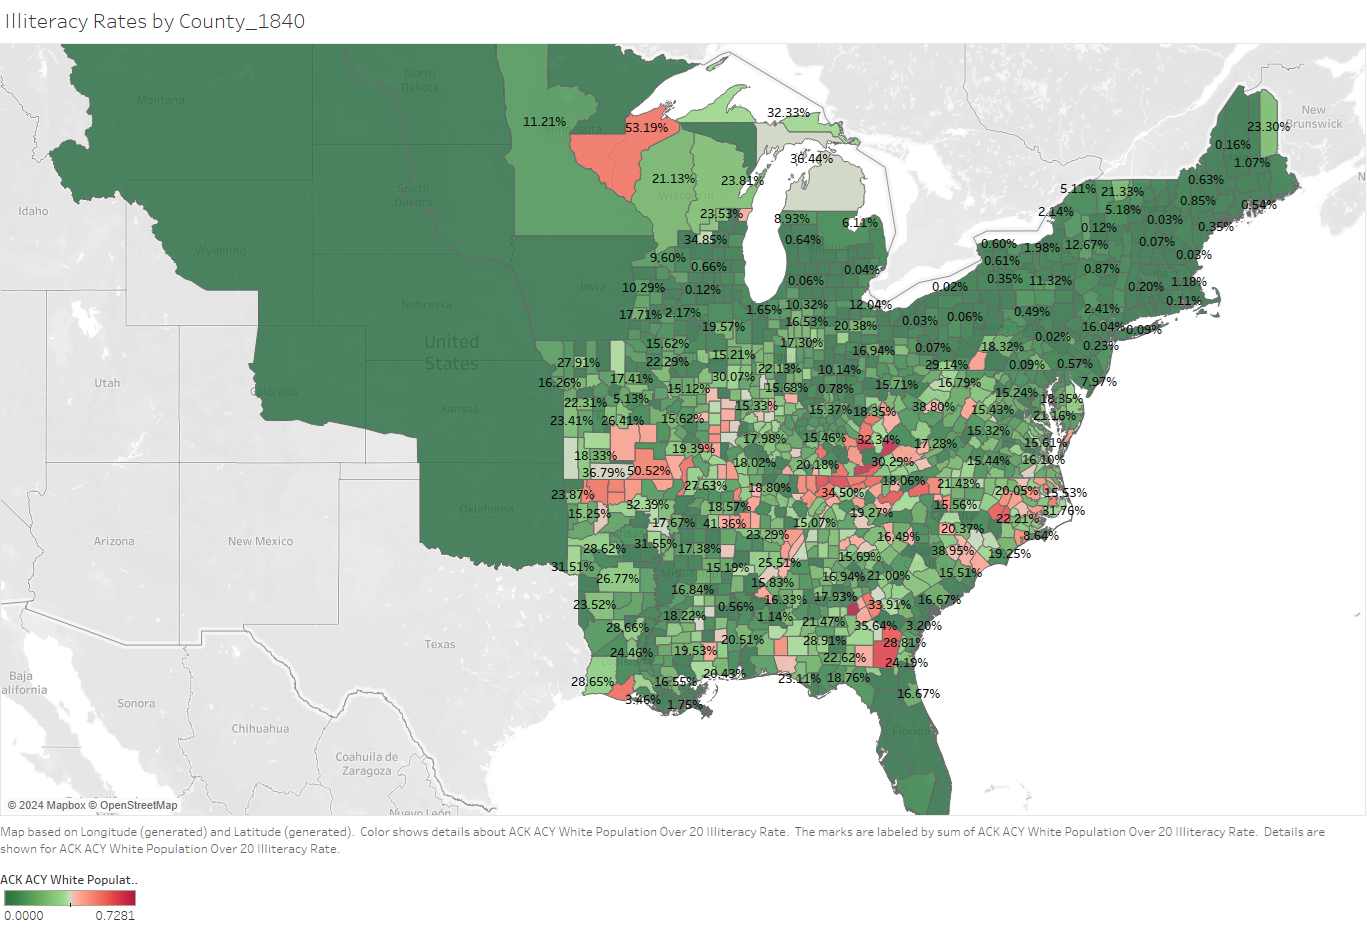
\includegraphics[width=\linewidth,height=\textheight,keepaspectratio]{IlliteracyRatesByCounty_1840.png}
    \caption{Geographic Visualization of the Response Variable ACKY}
    \label{fig:landscape_image}
\end{figure}
\end{landscape}


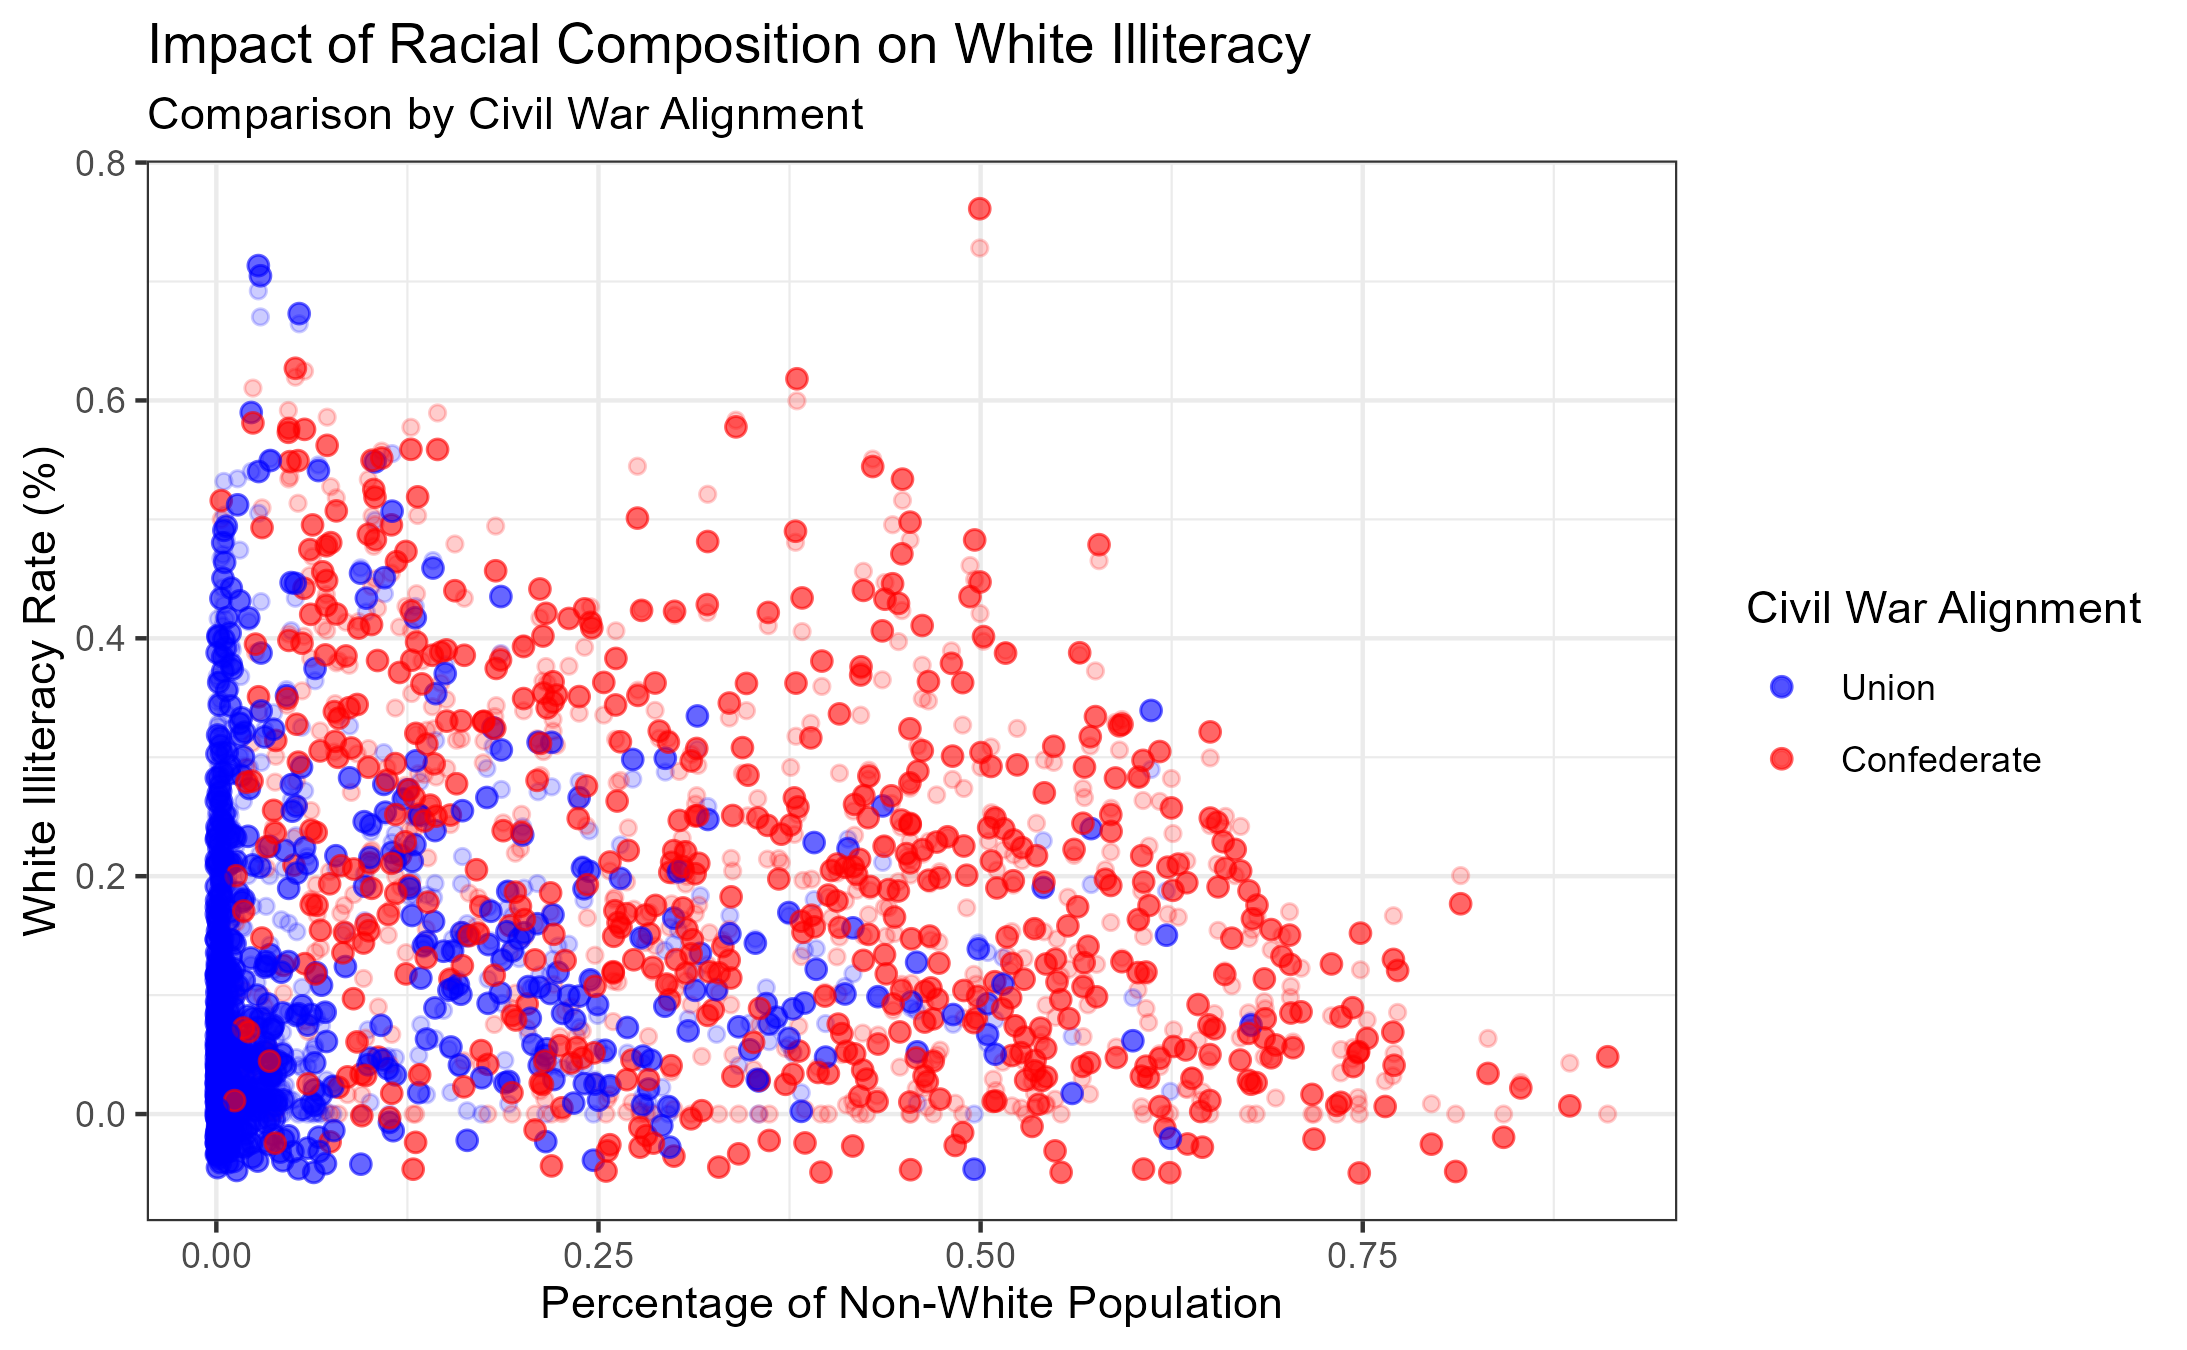
\includegraphics[scale=1]{ACSP.png}
\newline
The scatter plot of the racial composition helps explain the impact of a county's racial make-up on illiteracy rates.\* 

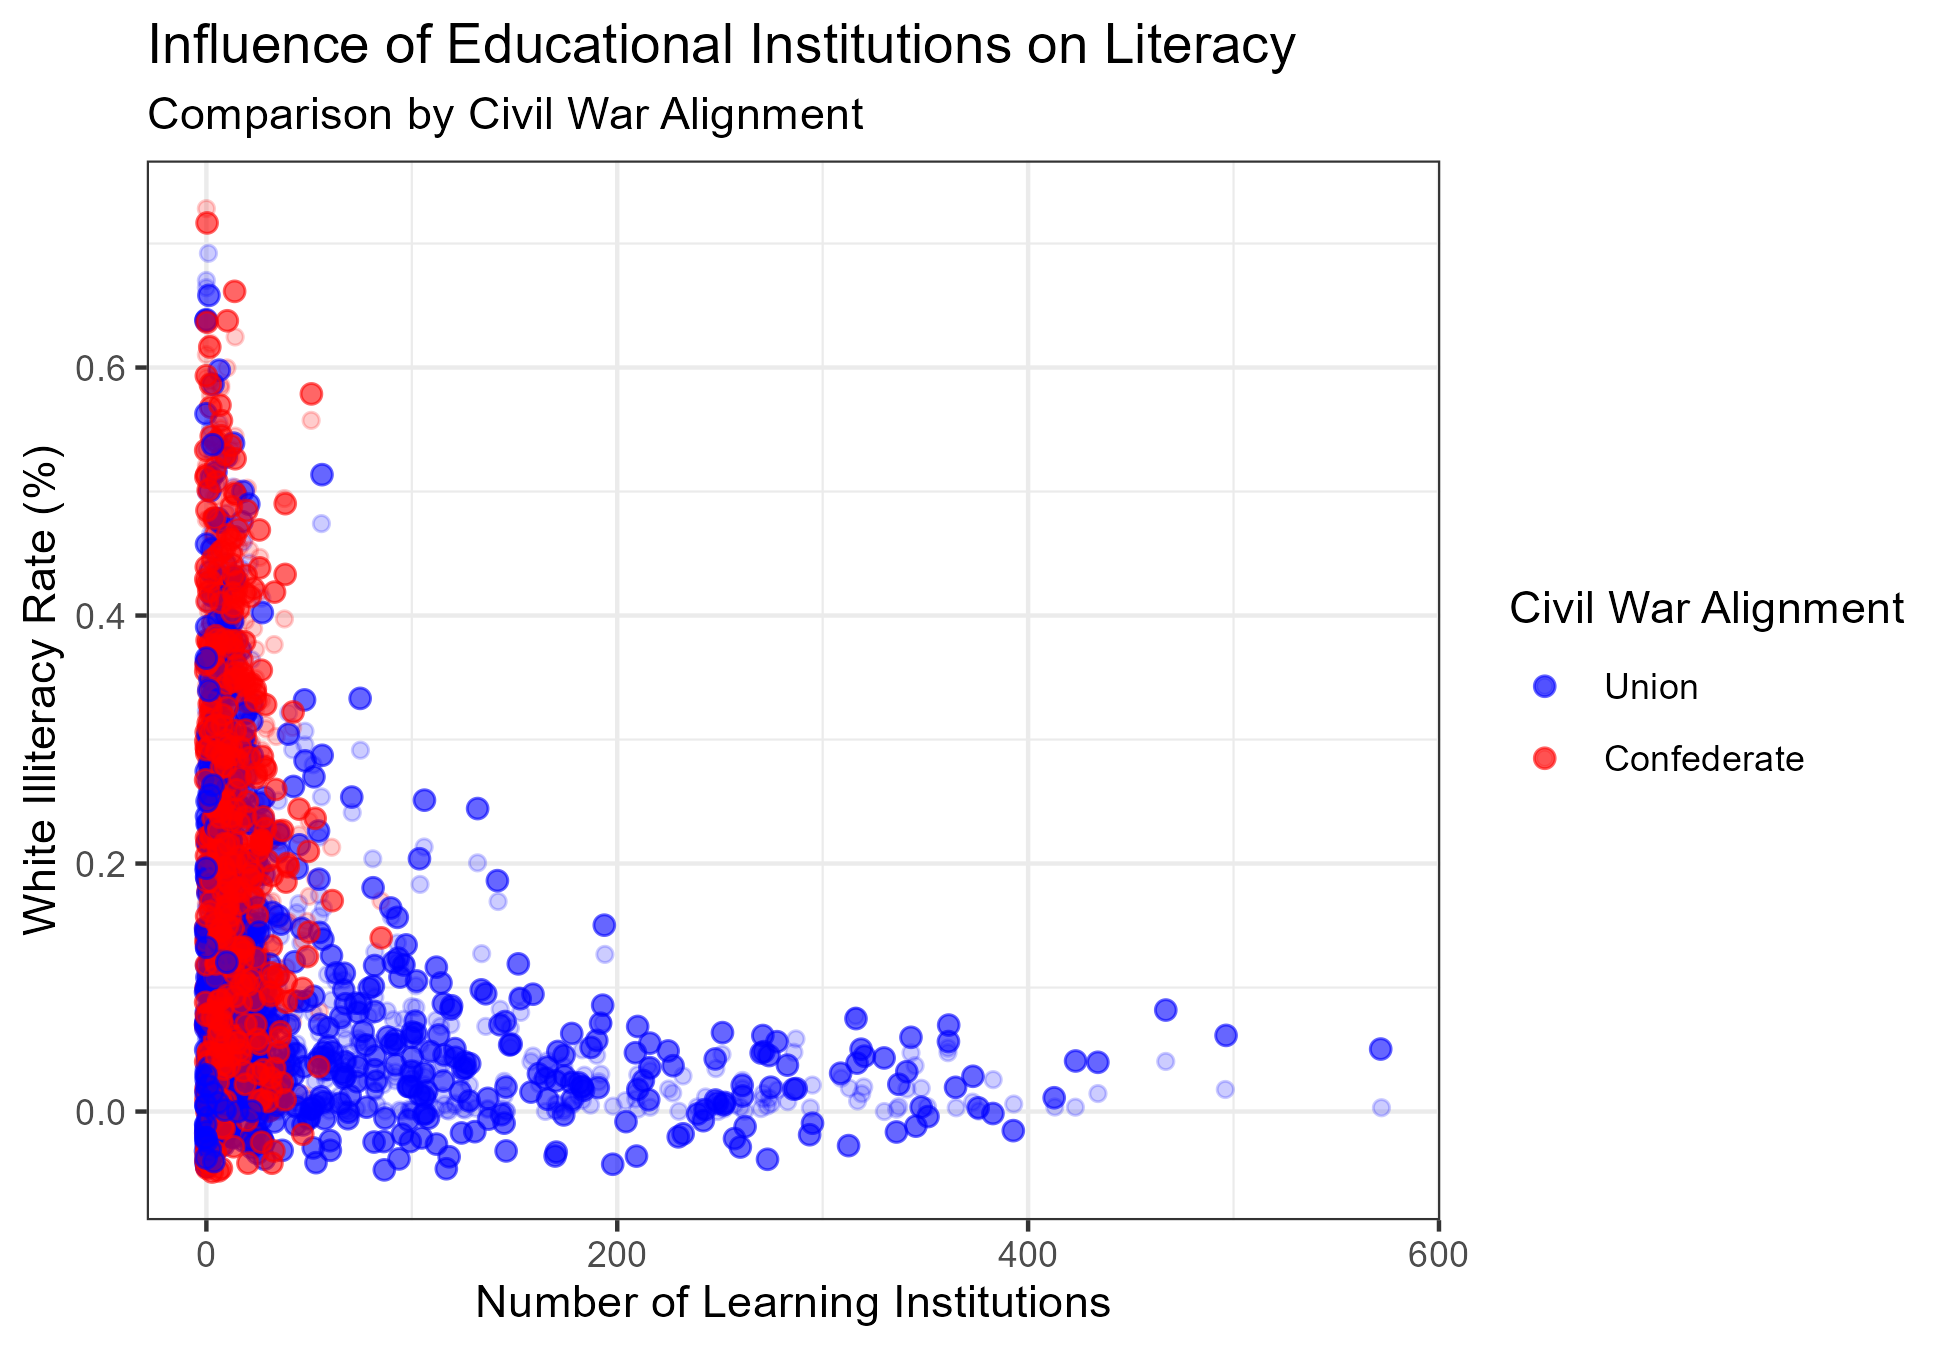
\includegraphics[scale=1]{ACH.png}
\newline


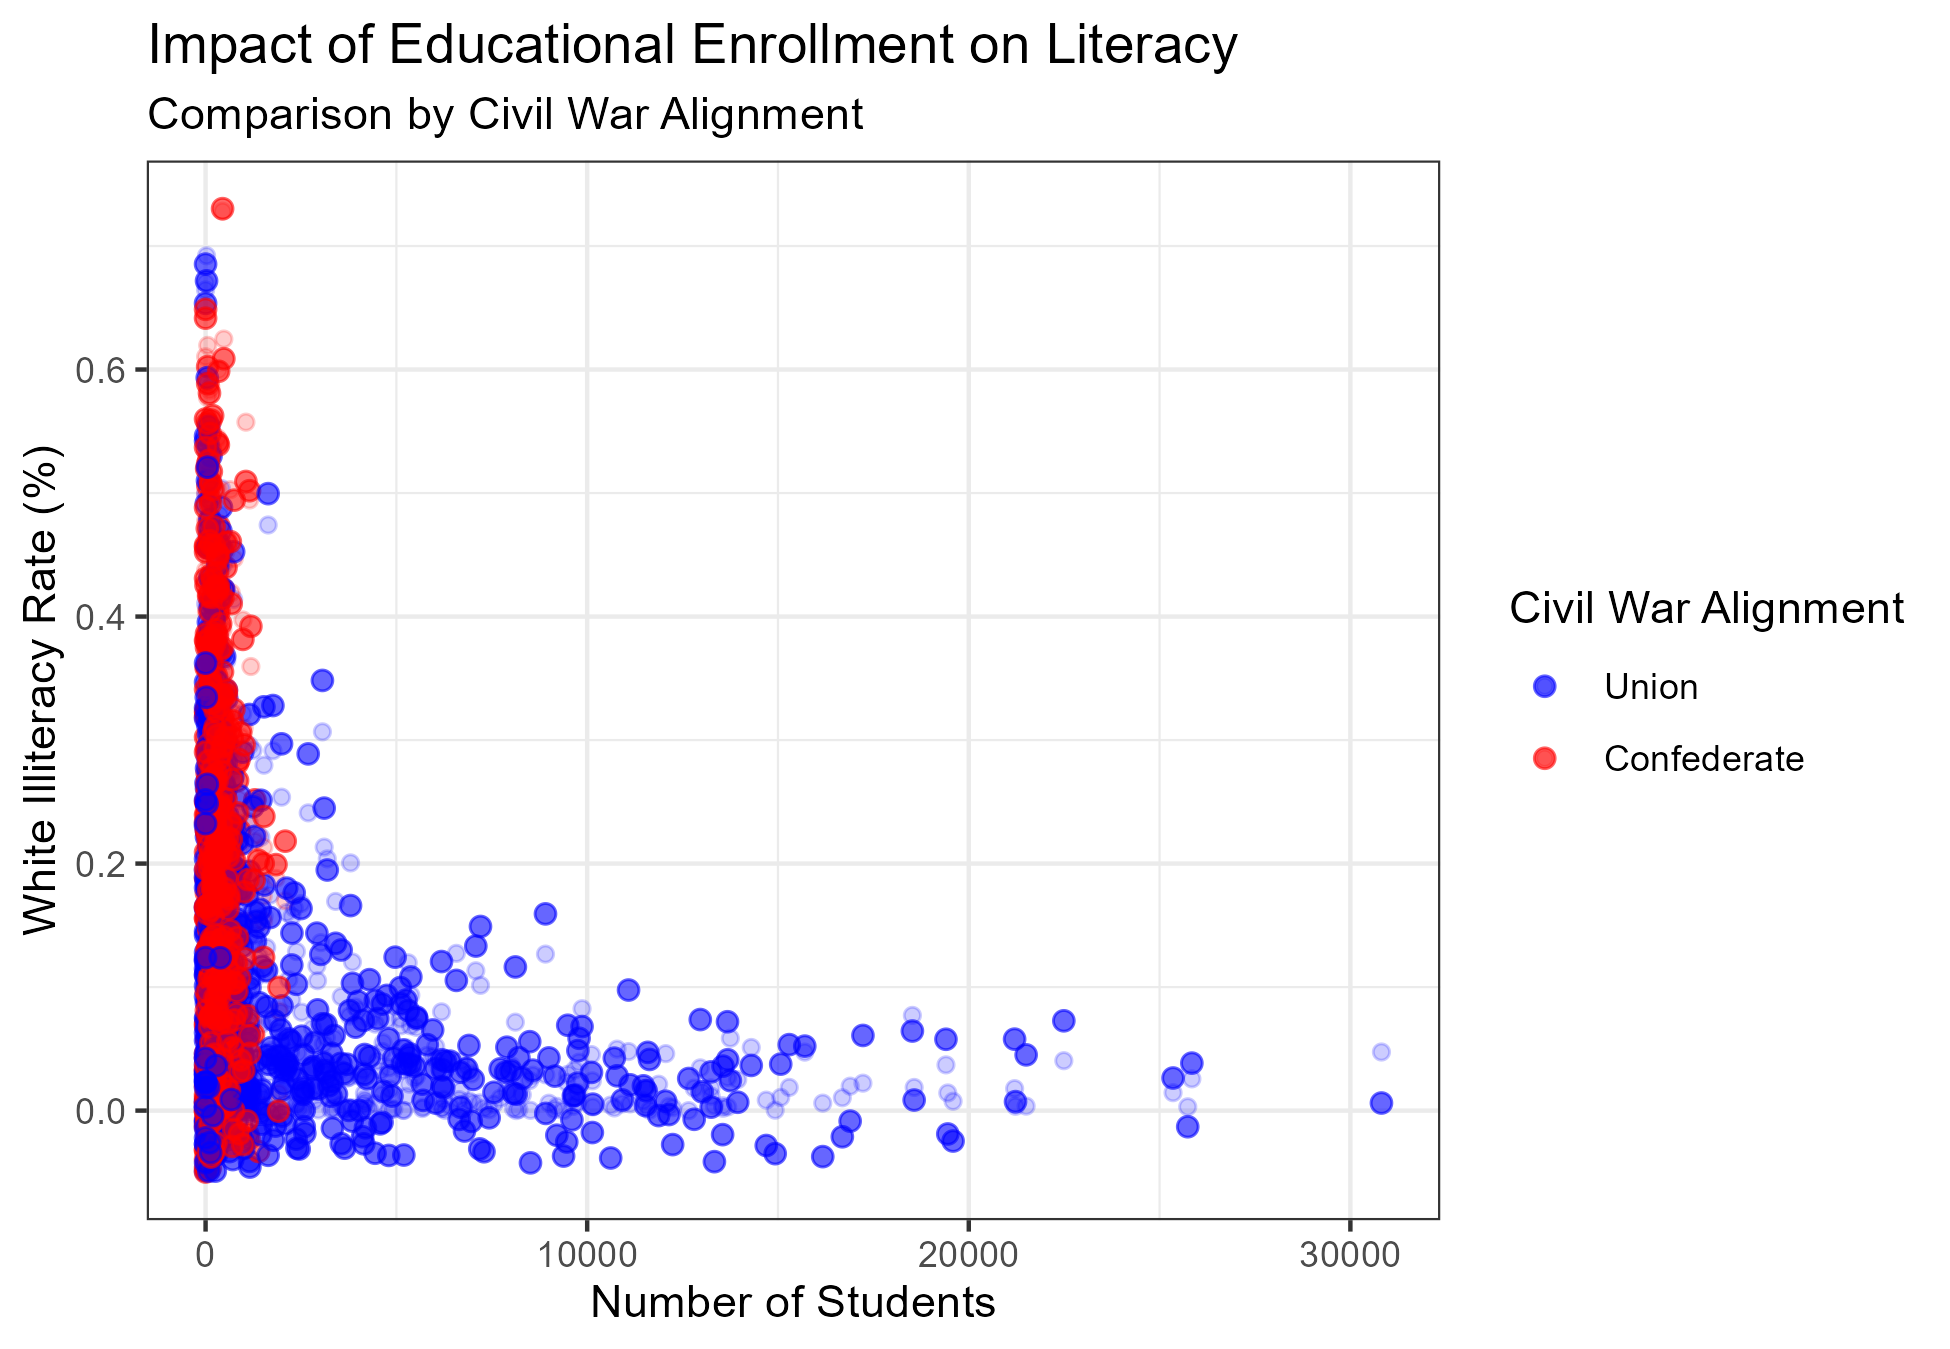
\includegraphics[scale=1]{ACI.png}
\newline


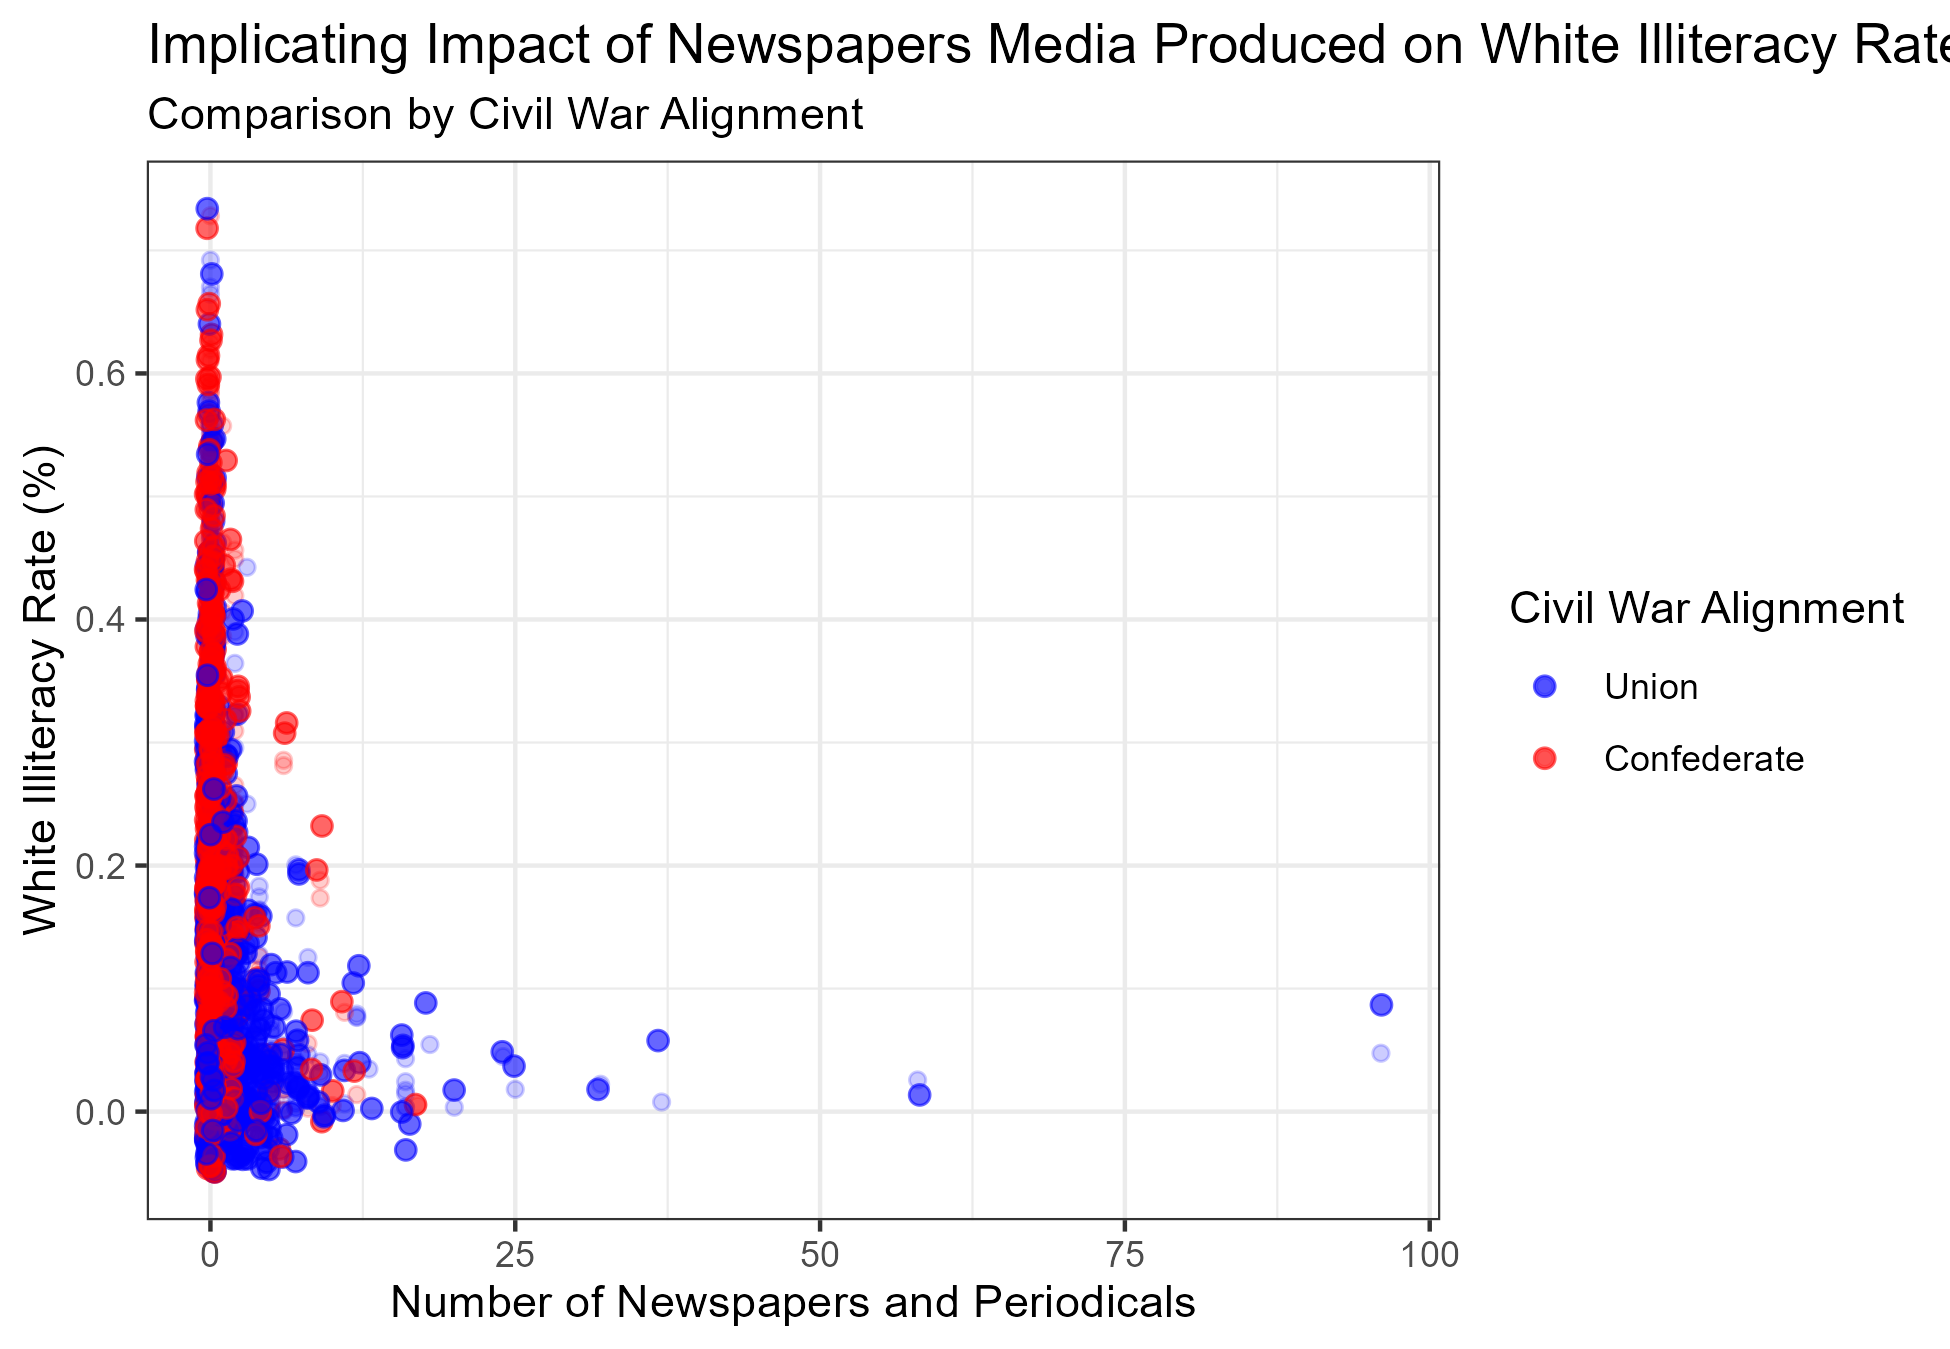
\includegraphics[scale=1]{ACM.png}
\newline


\end{document}

